\chapter{Convolutional Neural Network (CNN/ ConvNet) \cite{gfg-convolutional-neural-network-cnn-in-machine-learning}}\label{Convolutional Neural Network}

\begin{itemize}
    \item Convolutional Neural Networks, or CNNs, are a specialized class of neural networks designed to effectively process grid-like data, such as images.

    \item A Convolutional Neural Network (CNN) is a type of deep learning algorithm that is particularly well-suited for image recognition and processing tasks.
\end{itemize}


\section{Components}
\subsection{Kernel/ Filter}


\section{Layers}
\subsection{Convolutional Layer \cite{gfg-convolutional-neural-network-cnn-in-machine-learning}}\label{cnn: Convolutional layer}

\begin{itemize}
    \item These layers apply convolutional operations to input images, using filters (also known as kernels) to detect features such as edges, textures, and more complex patterns. 
    
    \item Convolutional operations help preserve the spatial relationships between pixels.
\end{itemize}


\subsection{Pooling Layer \cite{gfg-convolutional-neural-network-cnn-in-machine-learning}}\label{cnn: Pooling Layer}

\begin{itemize}
    \item Pooling layers \textbf{downsample} the spatial dimensions of the input, reducing the computational complexity and the number of parameters in the network. 
    
    \item Max pooling is a common pooling operation, selecting the maximum value from a group of neighboring pixels.

\end{itemize}

\subsubsection{Max Pooling \cite{gfg-cnn-introduction-to-pooling-layer}}\label{cnn: Max Pooling}

\begin{itemize}
    \item Max pooling is a pooling operation that selects the \textbf{maximum element} from the region of the feature map covered by the filter. 
    
    \item The output after max-pooling layer would be a feature map containing the \textbf{most prominent features} of the previous feature map.
\end{itemize}

\subsubsection{Average Pooling \cite{gfg-cnn-introduction-to-pooling-layer}}\label{cnn: Average Pooling}
\begin{itemize}
    \item Average pooling computes the \textbf{average of the elements} present in the region of feature map covered by the filter.
    
    \item Average pooling gives the average of features present in a patch.
\end{itemize}

\subsubsection{Global Pooling \cite{gfg-cnn-introduction-to-pooling-layer}}\label{cnn: Global Pooling}
\begin{itemize}
    \item Global pooling reduces each channel in the feature map to a single value.
    
    \item Thus, an $n_h \times n_w \times n_c$ feature map is reduced to $1 \times 1 x nc$ feature map. 

    \item This is equivalent to using a filter of dimensions $n_h \times n_w$ i.e. the dimensions of the feature map.
\end{itemize}

\begin{table}[h]
    \begin{minipage}[t]{0.32\linewidth}
        \begin{figure}[H]
            \centering
            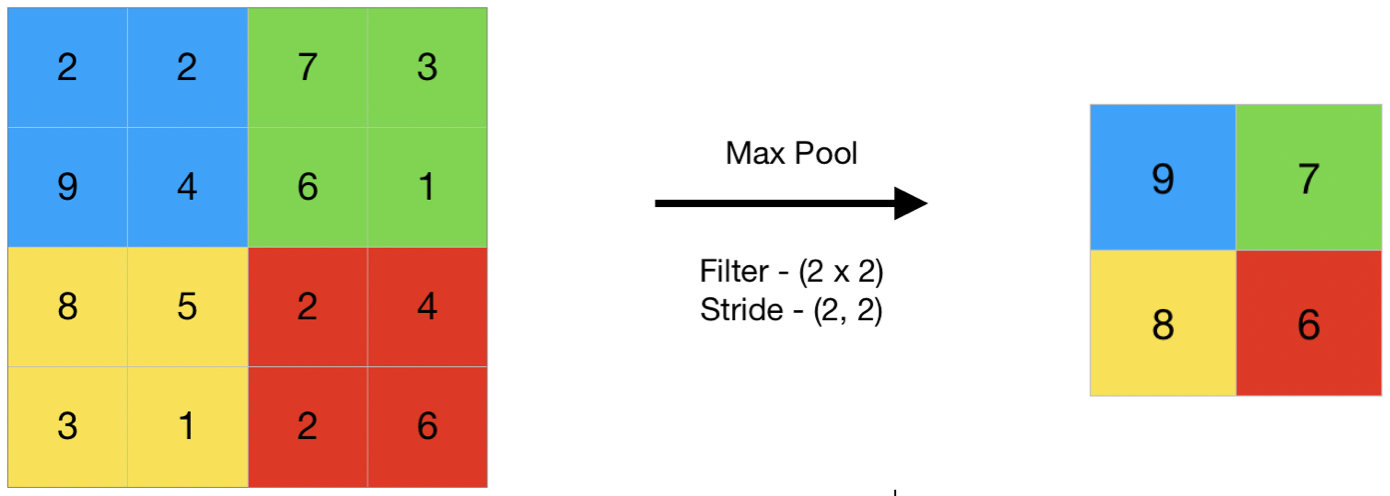
\includegraphics[width=\linewidth, height=4cm, keepaspectratio]{Pictures/convolutional-neural-network/pooling-max.png}
            \caption{Max Pooling}
        \end{figure}
    \end{minipage}
    \hfill
    \begin{minipage}[t]{0.32\linewidth}
        \begin{figure}[H]
            \centering
            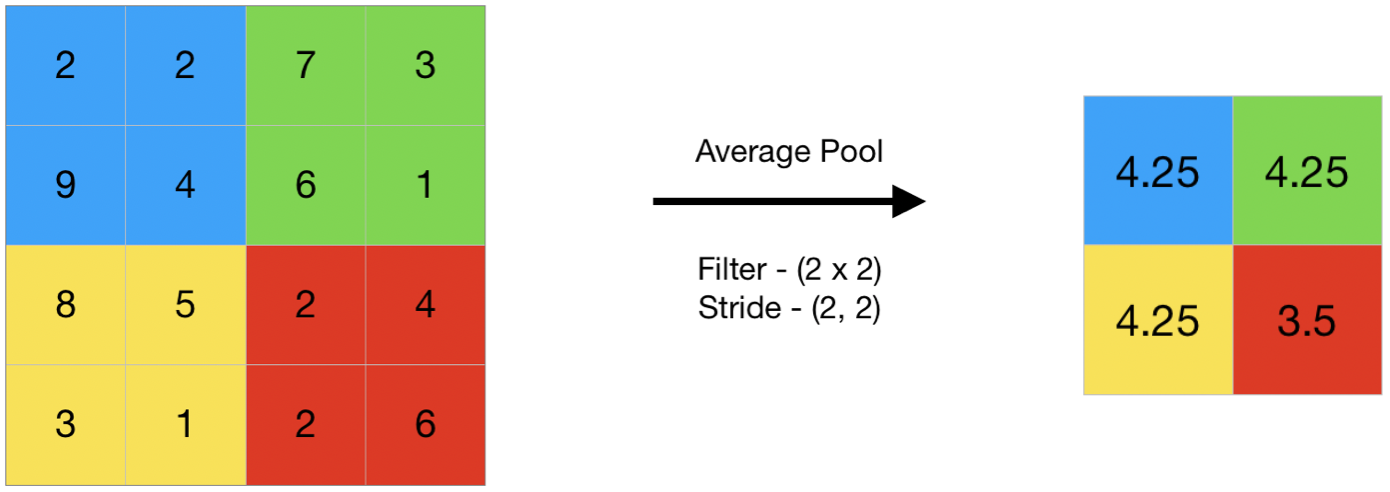
\includegraphics[width=\linewidth, height=4cm, keepaspectratio]{Pictures/convolutional-neural-network/pooling-average.png}
            \caption{Average Pooling}
        \end{figure}
    \end{minipage}
    \hfill
    \begin{minipage}[t]{0.32\linewidth}
        \begin{figure}[H]
            \centering
            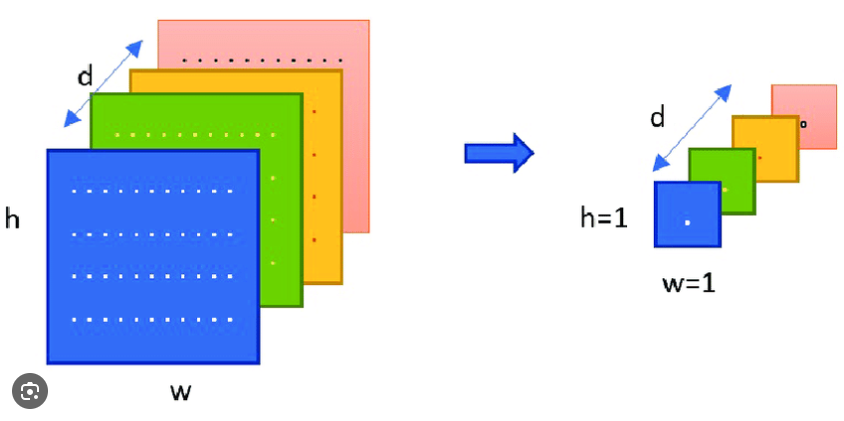
\includegraphics[width=\linewidth, height=4cm, keepaspectratio]{Pictures/convolutional-neural-network/pooling-global.png}
            \caption{Global Pooling}
        \end{figure}
    \end{minipage}
\end{table}


\subsection{Fully Connected Layer/ Dense Layer \cite{gfg-convolutional-neural-network-cnn-in-machine-learning}} \label{cnn: Fully Connected Layer/ Dense Layer}

\begin{itemize}
    \item These layers are responsible for making predictions based on the high-level features learned by the previous layers. 
    
    \item They connect every neuron in one layer to every neuron in the next layer.
\end{itemize}


\section{General Network Design \cite{gfg-convolutional-neural-network-cnn-in-machine-learning}}\label{cnn: General Network Design}

\begin{figure}[h]
    \centering
    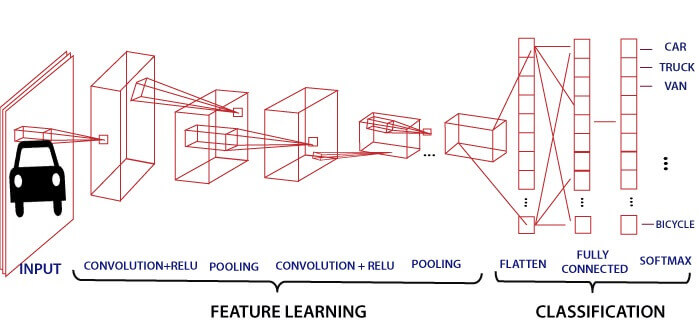
\includegraphics[width=\linewidth, height=5cm, keepaspectratio]{Pictures/convolutional-neural-network/convolutional-neural-network.jpg}
    \caption{CNN: General Network Design}
\end{figure}

\begin{itemize}
    \item The construction of a convolutional neural network is a multi-layered feed-forward neural network, made by assembling many unseen layers on top of each other in a particular order.

    \item It is the sequential design that give permission to CNN to learn hierarchical attributes.
    
    \item In CNN, some of them followed by grouping layers and hidden layers are typically convolutional layers followed by activation layers.
    
    \item The pre-processing needed in a ConvNet is kindred to that of the related pattern of neurons in the human brain and was motivated by the organization of the \textbf{Visual Cortex}.
\end{itemize}


\section{Formula}
\[
   \displaystyle n_{out} = \left[ \frac{n_{in} + 2p - k}{s} \right] + 1
\]

sometimes $k=f$

\begin{table}[h]
    \begin{minipage}[t]{0.5\linewidth}
        \begin{table}[H]
            \begin{tabular}{l l}
                $n_{in}$ & number of input features \\
                $n_{out}$ & number of output features \\
                $k$ & kernel size $k\times k$ / $(k, k)$ \\
                $p$ & padding size \\
                $s$ & stride size $s\times s$ / $(s, s)$ \\
            \end{tabular}
        \end{table}        
    \end{minipage}
    \hfill
    \begin{minipage}[t]{0.5\linewidth}
        \begin{table}[H]
            \begin{tabular}{l|l}
                \multicolumn{2}{c}{Padding Types}\\ \hline
                \textbf{Type} & $\mathbf{p}$ \textbf{value} \\ \hline
                Valid & 0 \\
                Same & \( \displaystyle p = \frac{k - 1}{2} \) \\
                
            \end{tabular}
        \end{table}        
    \end{minipage}
\end{table}






\vspace{5cm}
\url{https://www.geeksforgeeks.org/convolutional-neural-network-cnn-in-machine-learning/}


